\section{Dynamic Programming and the Linear Quadratic Regulator}

\subsection{The Optimal Control Problem}

In this section, we will outline the deterministic continuous-time optimal control problem that we will aim to solve. We will denote the state at time $t$ as $\st(t) \in \R^n$, and the control as $\ac(t) \in \R^m$. We will also occasionally write these as $\st_t$ and $\ac_t$, respectively. We will write the continuous-time systems dynamics as 
\begin{equation}
    \stdot(t) = \bm{\f}(\st(t),\ac(t),t).
    \label{eq:2_ct_dyn}
\end{equation}
We will refer to a history of control input values during an interval $[t_0,t_f]$ as a control history, and we will refer to a history of state values over this interval as a state trajectory. 

Different control problems may call for various constraints. For example, we may constrain a quadrotor to only fly in space not occupied by obstacles. Examples of constraints we will see are
\begin{itemize}
    \item Initial and final conditions, $\st(t_0) = \st_0$, $\st(t_f) = \st_f$
    \item Trajectory constraints, $\munderbar{\st} \leq \st(t) \leq \bar{\st}$
    \item Control limits, $\munderbar{\ac} \leq \ac(t) \leq \bar{\ac}$.
\end{itemize}
A state trajectory and control history that satisfy the constraints during the entire time interval $[t_0,t_f]$ are called admissible trajectories and admissible controls, respectively. 

Finally, we will define the performance measure, 
\begin{equation}
    J = \cost_f(\st(t_f),t_f) + \int_{t_0}^{t_f} \cost(\st(t),\ac(t),t) dt
    \label{eq:2_perf}
\end{equation}
where $\cost$ is the instantaneous cost function, and $\cost_f$ is the terminal state cost. We are now able to state the continuous-time optimal control problem. 
We aim to find an admissible control, $\ac^*$, which causes the system (\ref{eq:2_ct_dyn}) to follow an admissible trajectory, $\st^*$, that minimizes the performance measure given by (\ref{eq:2_perf}). The minimizer $(\st^*,\ac^*)$ is called an optimal trajectory-control pair. 

Note, first of all, that this is an extremely general problem formulation. We have not fixed our system dynamics, cost function, or specific constraints. We can't, in general, guarantee the existence or uniqueness of the optimal solution. 

There are two possible solution forms for the optimal control. The first, $\ac^* = e(\st(t_0),t)$ is referred to as an open-loop solution. This is an input function that is applied to the system, without using feedback. Practically, such solutions usually require augmentation with a feedback controller, as small model mismatch may lead to compounding errors. The second possible solution form is a feedback policy, $\ac^* = \pol(\st(t),t)$. This feedback law maps all state-time pairs to an action and thus is usually more robust to possible model mismatch. However, depending on the particular problem formulation, open-loop solutions may be easier to compute. 
% add discussion of discrete time optimal control problem?

\subsection{Dynamic Programming and the Principle of Optimality}


\begin{figure}[t]
    \centering
    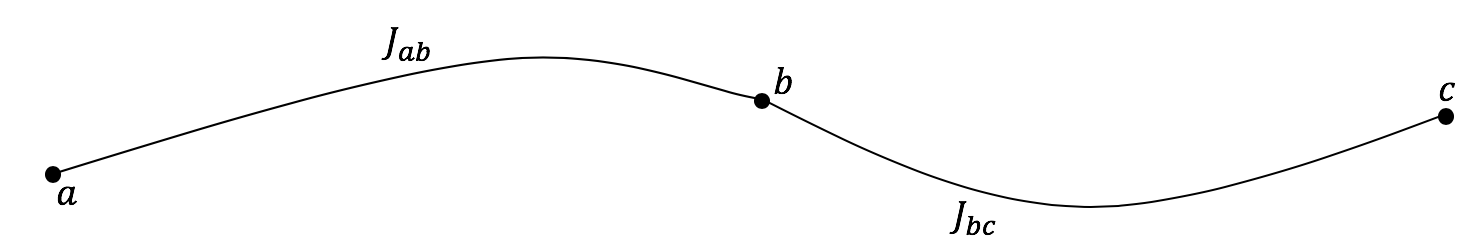
\includegraphics[width=0.8\linewidth]{figs/optimality.png}
    \caption{An optimal trajectory connecting point $a$ to point $c$. There are no better (lower cost) trajectories than the sub-trajectory connecting $b$ and $c$, by the principle of optimality.}
    \label{fig:opt1}
\end{figure}

In this chapter we will outline the principle of optimality, and the method of dynamic programming (DP), one of two main approaches to solving the optimal control problem. The second, so-called variational approaches based on Pontryagin's Maximum Principle (PMP) will be discussed in future chapters. Dynamic programming has the strong advantage of yielding a feedback policy, however, exactly solving the dynamic programming problem is infeasible for many systems. We will address special cases in which the DP problem can be solved exactly, and approximate methods that work for a wide variety of systems. 

Despite having just introduced the optimal control problem in continuous time, we will be operating in discrete time here, in which we aim to minimize 
\begin{equation}
    \J_f(\st_0) = \cost_f(\st_N) + \sum_{k=0}^{N-1} \cost(\st_k, \ac_k, k).
    \label{eq:disc_cost}
\end{equation}
We will extend the methods we develop in this chapter to continuous time in the next chapter. 

The principle of optimality is as follows. Figure \ref{fig:opt1} shows a trajectory from point $a$ to $c$. If the cost of the trajectory, $J_{ac} = J_{ab} + J_{bc}$, is minimal, then $J_{bc}$ is also a minimum cost trajectory connecting $b$ and $c$. The proof of this principle, stated informally, is simple. Assume there exists an alternative trajectory connecting $b$ and $c$, for which we will write the cost as $\tilde{J}_{bc}$, that achieves $\tilde{J}_{bc} < J_{bc}$. Then, we have 
\begin{align}
    \tilde{J}_{ac} &= J_{ab} + \tilde{J}_{bc}\\
    &< J_{ab} + J_{bc}\\
    &= J_{ac},
\end{align}
and thus $J_{ac}$ isn't minimal. More formally,

\begin{theorem}[Discrete-time Principle of Optimality]
Let $\pi^* = (\pi_0^*, \ldots, \pi^*_{N-1})$ be an optimal policy. Assume state $\st_k$ is reachable. Consider the subproblem whereby we are at $\st_k$ at time $k$ and we wish to minimize the cost-to-go from time $k$ to time $N$. Then the truncated policy $(\pi_k^*, \ldots, \pi^*_{N-1})$ is optimal for the subproblem.
\end{theorem}

Dynamic programming, intuitively, proceeds backwards in time, first solving simpler shorter horizon problems. If we have found the optimal policy for times $k+1$ to $N-1$, along with the associated cost-to-go for each state, choosing the optimal policy for time $k$ is a one step optimization problem. More concretely, we will assume we have dynamics of the form $\st_{k+1} = \f(\st_k,\ac_k,k)$ with $\ac_k \in \mathcal{U}(\st_k)$, and the cost given by (\ref{eq:disc_cost}). Then, dynamic programming iterates backward in time, from $N-1$ to $0$, with
\begin{align}
    \J_N(\st_N) &= \cost_T(\st_N)\\
    \J_k(\st_k) &= \min_{\ac_k \in \mathcal{U}(\st_k)} \left\{ \cost_k(\st_k,\ac_k,k) + \J_{k+1}(\f(\st_k,\ac_k,k)) \right\}.
    \label{eq:DP_rec}
\end{align}
Note that here we have considered only deterministic dynamical systems (there is no stochastic disturbance). Equation (\ref{eq:DP_rec}) is one form of the \textit{Bellman equation}, one of the most important relations in optimal control. 

Dynamic programming raises many practical issues if one were to attempt to apply it directly. To perform the recursion, $\J_{k+1}$ must be known for all $\st_{k+1}$ (or more precisely, all $\st_{k+1}$ that are reachable from $\st_k$). If the state space is discrete (and relatively small), this is tractable as the cost-to-go may just be maintained in tabular form. In the next subsection, we will discuss an extremely important case in continuous space in which the cost-to-go can be computed exactly for all states. However, for general systems, we can not expect to be able to compute the cost-to-go for all states. Possible approaches to make the DP approach tractable are discretizing the state space, approximating the cost-to-go (i.e. restricting the family of functions that $\J_{k+1}$ may be in), or interpolating between cost-to-go computed for a finite set of states. 

% should talk about the limitations of each of these methods

% should talk about how this yields a globally optimal, closed-loop policy

% add discrete DP example 

\subsection{Discrete LQR}
\label{sec:disrete_LQR}
An important instance in which dynamic programming can be solved analytically for continuous state-action systems is the \textit{linear quadratic regulator} problem. We will fix the dynamics of the system to be (possibly time-varying) linear, 
\begin{equation}
    \st_{k+1} = A_k \st_k + B_k \ac_k
\end{equation}
and the cost function as quadratic
\begin{align}
    \cost(\st_k, \ac_k) &= \frac{1}{2} ( \st_k^T Q_k \st_k + \ac_k^T R_k \ac_k )\\
    \cost_N(\st_k) &= \frac{1}{2} \st_k^T Q_N \st_k
\end{align}
where $Q_k \in \R^{n \times n}$ is positive semi-definite and $R_k \in \R^{m \times m}$ is positive definite for all $k = 0, \ldots, N$. Importantly, we assume $\st_k$ and $\ac_k$ are unconstrained for all $k$. To perform DP recursion, we initialize 
\begin{equation}
    \J_N^*(\st_N) = \frac{1}{2} \st_N^T Q_N \st_N \vcentcolon= \frac{1}{2} \st_N^T V_N \st_N.
\end{equation}
Then, applying (\ref{eq:DP_rec}), we have
\begin{equation}
    \J_{N-1}^*(\st_{N-1}) = \frac{1}{2} \min_{\ac_{N-1} \in \R^m} \left\{ \st_{N-1}^T Q_{N-1} \st_{N-1} + \ac_{N-1}^T R_{N-1} \ac_{N-1} + \st_N^T V_N \st_N \right\}
\end{equation}
which, applying the dynamics,
\begin{align}
\label{eq:LQR_rec_cost}
    \J_{N-1}^*(\st_{N-1}) = \frac{1}{2} \min_{\ac_{N-1} \in \R^m} & {\large\{} \st_{N-1}^T Q_{N-1} \st_{N-1} + \ac_{N-1}^T R_{N-1} \ac_{N-1}\\
    &+ (A_{N-1} \st_{N-1} + B_{N-1} \ac_{N-1})^T V_N (A_{N-1} \st_{N-1} + B_{N-1} \ac_{N-1}) {\large\}}. \nonumber
\end{align}
Rearranging, we have
\begin{align}
    \J_{N-1}^*(\st_{N-1}) = \frac{1}{2} \min_{\ac_{N-1} \in \R^m} {\large\{}
    & \st_{N-1}^T (Q_{N-1} + A_{N-1}^T V_N A_{N-1}) \st_{N-1}\\ \nonumber
    & + \ac_{N-1}^T (R_{N-1} + B_{N-1}^T V_N B_{N-1}) \ac_{N-1}\\\nonumber
    & + 2 \ac_{N-1}^T (B_{N-1}^T V_N A_{N-1}) \st_{N-1} \nonumber
    {\large\}}.
\end{align}
Note that this optimization problem is convex in $\ac_{N-1}$ as $R_{N-1} + B_{N-1}^T V_N B_{N-1} > 0$. Therefore, any local minima is a global minima, and therefore we can simply apply the first order optimality conditions. Differentiating,
\begin{equation}
    \frac{\partial \J_{N-1}^*(\st_{N-1})}{\partial \ac_{N-1}} = (R_{N-1} + B_{N-1}^T V_N B_{N-1}) \ac_{N-1} + (B_{N-1}^T V_N A_{N-1}) \st_{N-1}
\end{equation}
and setting this to zero yields
\begin{equation}
    \ac^*_{N-1} = - (R_{N-1} + B_{N-1}^T V_N B_{N-1})^{-1} (B_{N-1}^T V_N A_{N-1}) \st_{N-1}
\end{equation}
which we write
\begin{equation}
    \ac^*_{N-1} = L_{N-1} \st_{N-1}
\end{equation}
which is a time-varying linear feedback policy. Plugging this feedback policy into (\ref{eq:LQR_rec_cost}),
\begin{align}
    \J_{N-1}^*(\st_{N-1}) =& \st_{N-1}^T (Q_{N-1}  + L_{N-1}^T R_{N-1} L_{N-1} \\
    & + (A_{N-1} + B_{N-1} L_{N-1})^T V_N   (A_{N-1} + B_{N-1} L_{N-1})) \st_{N-1}. \nonumber
\end{align}
Critically, this implies that the cost-to-go is always a positive semi-definite quadratic function of the state. Because the optimal policy is always linear, and the optimal cost-to-go is always quadratic, the DP recursion may be recursively performed backward in time and the minimization may be performed analytically. 

Following the same procedure, we can write the DP recursion for the discrete-time LQR controller:
\begin{enumerate}
    \item $V_N= Q_N$
    \item $L_k = - (R_{k} + B_{k}^T V_{k+1} B_{k})^{-1} (B_{k}^T V_{k+1} A_{k})$
    \item $V_{k} = Q_{k}  + L_{k}^T R_{k} L_{k} + (A_{k} + B_{k} L_{k})^T V_{k+1}   (A_{k} + B_{k} L_{k})$
    \item $\ac^*_k = L_k \st_k$
    \item $\J^*_k(\st_k) = \frac{1}{2} \st_k^T V_k \st_k$
\end{enumerate}
There are several implications of this recurrence relation. First, even if $A,B,Q,R$ are all constant (not time-varying), the policy is still time-varying. Why is this the case? Control effort invested early in the problem will yield dividends over the remaining length of the horizon, in terms of lower state cost for all future time steps. However, as the remaining length of the episode becomes shorter, this tradeoff is increasingly imbalanced, and the control effort will decrease. 
However, for a linear time-invariant system, if $(A,B)$ is controllable, the feedback gain $L_k$ approach a constant as the episode length approaches infinity. This time-invariant policy is practical for long horizon control problems, and may be approximately computed by running the DP recurrence relation until approximate convergence. 

\subsubsection{LQR with (Bi)linear Cost and Affine Dynamics}

In the previous subsection, we have derived the common formulation of the LQR controller. In this subsection, we will derive the discrete time LQR controller for a more general system with bilinear/linear terms in the cost and affine terms in the dynamics. This derivation will be the basis of algorithms we will build up in the following subsections. More concretely, we consider systems with stage-wise cost
\begin{equation}
    \cost(\st_k, \ac_k) = \frac{1}{2} \st_k^T Q_k \st_k + \frac{1}{2} \ac_k^T R_k \ac_k + \ac_k^T H_k \st_k +\bm{q}_k^T \st_k + \bm{r}_k \ac_k + q_k,
\end{equation}
terminal cost
\begin{equation}
    \cost_N(\st_k) = \frac{1}{2} \st_k^T Q_N \st_k + \bm{q}_N^T \st_k + q_N,
\end{equation}
and dynamics
\begin{equation}
    \st_{k+1} = A_k \st_k + B_k \ac_k + d_k.
\end{equation}
The cost-to-go will take the form 
\begin{equation}
    J_k(\st_k) = \frac{1}{2}\st_k^T V_k \st_k + \bm{v}_k^T \st_k + v_k.
\end{equation} 
Repeating our approach from the last subsection, we have
\begin{align}
\label{eq:LQR_rec_cost}
    \J_{k}^*(\st_{k}) =  \min_{\ac_{k} \in \R^m} & {\large\{} 
    \frac{1}{2} \st_{k}^T Q_{k} \st_{k} + \frac{1}{2} \ac_{k}^T R_{k} \ac_{k} + \ac_k^T H_k \st_k +\bm{q}_k^T \st_k + \bm{r}_k \ac_k + q_k \\
    &+ \frac{1}{2} (A_{k} \st_{k} + B_{k} \ac_{k} + \bm{d}_k)^T V_{k+1} (A_{k} \st_{k} + B_{k} \ac_{k} + \bm{d}_k) \nonumber \\
    & + \bm{v}^T_{k+1} (A_{k} \st_{k} + B_{k} \ac_{k} + \bm{d_k}) + v_{k+1} {\large\}}. \nonumber
\end{align}
Rearranging, have
\begin{align}
    \J_{k}^*(\st_{k}) = \min_{\ac_{k} \in \R^m} {\Large\{}  
    & \frac{1}{2} \st_k^T (Q_k + A_k^T V_{k+1} A_k) \st_k + \frac{1}{2} \ac_k^T (R_k + B_k^T V_{k+1} B_k) \ac_k\\
    & + \ac_k^T (H_k + B_k^T V_{k+1} A_k)^T \st_k + (\bm{q}_k + A_k^T V_{K+1} \bm{d}_k + A_k^T \bm{v}_{k+1})^T \st_k \nonumber \\
    & + (\bm{r}_k + B_k^T V_{k+1} \bm{d} + B_k^T \bm{v}_{k+1}) \ac_k + (v_{k+1} + \frac{1}{2} \bm{d}_k^T V_{k+1} \bm{d}_k + \bm{v}_{k+1}^T \bm{d}_k) \nonumber
    {\Large\}}.
\end{align}
Solving this minimization problem, we see that our optimal controller takes the form
\begin{equation}
    \ac^*_{k} =\bm{l}_k +  L_{k} \st_{k}.
\end{equation}
We will define the following useful terms which will be used throughout the remainder of this section
\begin{align}
\label{eq:Qk_lqr}
    % Q_k &= q_k + v_{k+1}\\
    % Q_{\st,k} &= \bm{q}_k + A_k^T \bm{v}_{k+1}\\
    S_{\ac,k} &= \bm{r}_k + B_k^T \bm{v}_{k+1} + B_k^T V_{k+1} \bm{d}_k\\
    % Q_{\st \st,k} &= Q_k + A_k^T V_{k+1} A_k\\
    S_{\ac \ac,k} &= R_k + B_k^T V_{k+1} B_k\\
    S_{\ac \st,k} &= H_k + B_k^T V_{k+1} A_k.
\end{align}
Given this notation, all necessary terms can be computed via the following relations
\begin{enumerate}
    \item $V_N = Q_N$; $\bm{v}_N = \bm{q}_N$; $v_N = q_N$
    \item \begin{align} L_k &= - S_{\ac \ac,k}^{-1} S_{\ac \st,k}\\
    \bm{l}_k &= - S_{\ac \ac,k}^{-1} S_{\ac,k}
    \end{align}
    \item 
    % \begin{align}
    %     V_k &= Q_{k}  + L_{k}^T (R_k L_k + H_k) + (A_K + B_k L_k)^T V_{k+1} (A_K + B_k L_k)\\
    %     \bm{v}_k &= \bm{q}_k + L_{k}^T (R_k \bm{l}_k + \bm{r}_k) + H_k^T \bm{l}_k + (A_K + B_k L_k)^T (V_{k+1} (B_k \bm{l}_k + \bm{d}_k) + \bm{v}_{k+1}) \\
    %     v_k &= v_{k+1} + q_k + \bm{l}_{k}^T \bm{r}_k + (B_k \bm{l}_k + \bm{d}_k)^T \bm{v}_{k+1} + \frac{1}{2} (\bm{l}_k^T R_k \bm{l}_k + (B_k \bm{l}_k + \bm{d}_k)^T V_{k+1} (B_k \bm{l}_k + \bm{d}_k))
    % \end{align}
    \begin{align}
        V_k &= Q_{k}  + A_k^T V_{k+1} A_k - L_k^T S_{\ac \ac,k} L_k\\
        \bm{v}_k &= \bm{q}_k + A_k^T (\bm{v}_{k+1} + V_{k+1} \bm{d}_k) + S_{\ac \st,k} \bm{l}_k + L_k^T (S_{\ac,k} + S_{\ac \ac,k} \bm{l}_k) \\
        v_k &= v_{k+1} + q_k + \bm{d}_k^T \bm{v}_{k+1} + \frac{1}{2} \bm{d}_k^T V_{k+1} \bm{d}_k + \bm{l}_k^T (S_{\ac,k} + \frac{1}{2} S_{\ac \ac,k} \bm{l}_k)
    \end{align}
    \item $\ac^*_{k} =\bm{l}_k +  L_{k} \st_{k}$
    \item $J_k(\st_k) = \frac{1}{2}\st_k^T V_k \st_k + \bm{v}_k^T \st_k + v_k$.
\end{enumerate}
Note that in the following subsections (specifically in our discussion of differential dynamic programming) we will introduce more convenient (and compact) notation. 

\subsubsection{LQR Tracking around a Linear Trajectory}

In the previous subsections we have considered the generic linear quadratic control problem, in which we want to regulate to a fixed point, and deviations from this point are penalized. In this section, we will address the case in which we want to track a pre-specified trajectory. Let us assume (for now) that we have been given a nominal trajectory of the form $(\bar{\st}_0, \ldots, \bar{\st}_{N})$ and $(\bar{\ac}_0, \ldots, \bar{\ac}_{N-1})$. We will also assume that this trajectory satisfies our given dynamics, such that 
\begin{equation}
\bar{\st}_{k+1} = A_k \bar{\st}_k + B_k \bar{\ac}_k + \bm{d}_k,\,\, \forall k = 0, \ldots, N-1.    
\end{equation}
Then, we can rewrite our dynamics in terms of deviations from the nominal trajectory, 
\begin{align}
    \delta \st_k &= \st_k - \bar{\st}_k\\
    \delta \ac_k &= \ac_k - \bar{\ac}_k.
\end{align}
Rewriting, we have 
\begin{equation}
    \delta \st_{k+1} = A_k \delta \st_k + B_k \delta \ac_k.
\end{equation}
Thus, tracking the nominal trajectory reduces to driving the state deviation, $\delta \st_k$, to zero. Note that solving this problem requires rewriting the original cost function in terms of the deviations $\delta \st_k, \delta \ac_k$. 

% should expand discussion -- possibly write out the modified cost function?

\subsubsection{LQR Tracking around a Nonlinear Trajectory}

Despite LQR being an extremely powerful approach to optimal control, it suffers from a handful of limitations. First and foremost, it assumes the dynamics are (possibly time-varying) linear, and the cost function is quadratic. While most systems are in fact nonlinear, a typical approach to designing feedback controllers is to linearize around some operating point. This is an effective method for designing regulators, which aim to control the system to some particular state. If, in contrast, we wish to track a trajectory, we must instead linearize around this trajectory. We will assume we are given a nominal trajectory which satisfies the nonlinear dynamics, such that
\begin{equation}
    \bar{\st}_{k+1} = \f(\bar{\st}_k,\bar{\ac}_k),\,\, \forall k = 0, \ldots, N-1. 
\end{equation}
Given this, we can linearize our system at each timestep by Taylor expanding,
\begin{equation}
    \st_{k+1} \approx \f(\bar{\st}_k,\bar{\ac}_k) + \underbrace{\frac{\partial \f}{\partial \st} (\bar{\st}_k, \bar{\ac}_k)}_{A_k} (\st_k - \bar{\st}_k) + \underbrace{\frac{\partial \f}{\partial \ac} (\bar{\st}_k, \bar{\ac}_k)}_{B_k} (\ac_k - \bar{\ac}_k).
\end{equation}
which allows us to again rewrite the system in terms of deviations, to get
\begin{equation}
    \delta \st_{k+1} = A_k \delta \st_k + B_k \delta \ac_k
\end{equation}
which is linear in $\delta \st_k, \delta \ac_k$.  Note that design of systems of this type often require careful design and analysis, as deviating from the nominal trajectory results in the loss of accuracy of the local model linearization. 

In designing this tracking system, a second question now occurs: how do we choose our cost function? One possible option is arbitrary choice of $Q$ and $R$ by the system designer. This has the advantage of being easily customizable to change system behavior, and we can guarantee the necessary conditions on these matrices. A second option, if we are given some arbitrary (possibly non-quadratic) cost function $\cost$, is to locally quadratize the cost function. Writing 
\begin{align}
    \label{eq:cost_derivs}
    \cost_{k} &\vcentcolon= \cost(\bar{\st}_k,\bar{\ac}_k)\\
    \cost_{i,k} &\vcentcolon= \frac{\partial \cost}{\partial i}(\bar{\st}_k,\bar{\ac}_k)\\
    \cost_{ij,k} &\vcentcolon= \frac{\partial^2 \cost}{\partial i \partial j}(\bar{\st}_k,\bar{\ac}_k)
\end{align}
we can second order Taylor expand our cost function around our nominal trajectory
\begin{equation}
    \cost(\delta \st_k, \delta \ac_k) \approx 
\frac{1}{2}
    \begin{bmatrix}
    1\\
    \delta \st_k\\
    \delta \ac_k
\end{bmatrix}^T
    \begin{bmatrix}
    2 \cost_k & \cost_{\st,k}^T & \cost_{\ac,k}^T\\
    \cost_{\st,k} & \cost_{\st \st,k} & \cost_{\ac \st,k}^T\\
    \cost_{\st,k} & \cost_{\ac \st,k} & \cost_{\ac \ac,k}
\end{bmatrix}
    \begin{bmatrix}
    1\\
    \delta \st_k\\
    \delta \ac_k
\end{bmatrix}.
\label{eq:cost_qf}
\end{equation}
Here $\cost_{\st \st,k}$ and $\cost_{\ac \ac,k}$ replace $Q_k$ and $R_k$ from the previous section, respectively. There are two primary concerns with this approach to choosing the cost function. First, we require the quadratic form in (\ref{eq:cost_qf}) to be positive semi-definite and $\cost_{\ac \ac,k}$ to be positive definite, for all $k$. Second, we have an implicit cost that we would like to stay close to the nominal trajectory to ensure our linearized model does not become inaccurate. As a result of this implicit cost, we may wish to tune the cost terms to yield tracking that is better suited to the nonlinear model that we are tracking. 

\subsection{Iterative LQR and Differential Dynamic Programming}

\subsubsection{Iterative LQR}

We have addressed the case in which we wish to track a given trajectory with LQR. A natural question, now, is whether we can use LQR to improve on this nominal trajectory? Iterative LQR augments tracking LQR with a forward pass in which the nominal trajectory is updated. As a consequence, it can be used to improve trajectories and in most cases, can be used as a practical trajectory generation and control algorithm for nonlinear systems. We will define the following useful terms
%double check if multipliers on constant terms are correct
\begin{align}
\label{eq:Qk}
    Q_k &= \cost_k + v_{k+1}\\
    Q_{\st,k} &= \cost_{\st,k} + \f_{\st,k}^T \bm{v}_{k+1}\\
    Q_{\ac,k} &= \cost_{\ac,k} + \f_{\ac,k}^T \bm{v}_{k+1}\\
    Q_{\st \st,k} &= \cost_{\st \st,k} + \f_{\st,k}^T V_{k+1} \f_{\st,k} \label{eq:Qxxk}\\
    Q_{\ac \ac,k} &= \cost_{\ac \ac,k} + \f_{\ac,k}^T V_{k+1} \f_{\ac,k}\\
    Q_{\ac \st,k} &= \cost_{\ac \st,k} + \f_{\ac,k}^T V_{k+1} \f_{\st,k} \label{eq:Quxk}
\end{align}
where $\f_{\st,k} = A_k$ and $\f_{\ac,k} = B_k$. In this form, the optimal control perturbation is
\begin{equation}
    \delta \ac_k^* = \bm{l}_k + L_k \delta \st_k
\end{equation}
where 
\begin{align}
    \label{eq:iLQR_fb1}
    \bm{l}_k &= - Q_{\ac \ac,k}^{-1} Q_{\ac,k}\\
    L_k &= - Q_{\ac \ac,k}^{-1} Q_{\ac \st,k}. \label{eq:iLQR_fb2}
\end{align}

Finally, the local backward recursion can be completed by updating the value function terms via
\begin{align}
    \label{eq:iLQR_V1}
    V_k &= Q_k - \frac{1}{2} \bm{l}_k^T Q_{\ac \ac, k} \bm{l}_k\\
    V_{\st_k} &= Q_{\st,k} - L_k^T Q_{\ac \ac, k} \bm{l}_k\\
    V_{\st \st, k} &= Q_{\st \st,k} - L_k^T Q_{\ac \ac, k} L_k. \label{eq:iLQR_V3}
\end{align}

\begin{algorithm}[t]
\caption{iLQR}
\centering
\label{alg:iLQR}

%\begin{minipage}[t]{0.5\textwidth}
\begin{algorithmic}[1]
\Require Nominal control sequence, $(\bar{\ac}_0, \ldots, \bar{\ac}_{N-1})$
    \State $\delta \ac_k = 0$ for all $k$ 
    \While{not converged}
    \Statex Forward pass:
    \State Compute nominal trajectory $\bar{\st}_{k+1} = \f(\bar{\st}_k, \bar{\ac}_k + \delta \ac_k)$ and set $\bar{\ac}_k \gets \bar{\ac}_k + \delta \ac_k$
    \Statex Backward pass:
    \State Compute $Q$ terms around $(\bar{\st}_k, \bar{\ac}_k)$ for all $k$ via (\ref{eq:Qk} -- \ref{eq:Quxk})
    \State Update feedback law via (\ref{eq:iLQR_fb1} -- \ref{eq:iLQR_fb2})
    \State Update value approximation via (\ref{eq:iLQR_V1} -- \ref{eq:iLQR_V3})
    \EndWhile
    \State Compute control law $\pol_k(\st_k) = \bar{\ac}_k + \bm{l}_k + L_k(\st_k - \bar{\st}_k)$
    \State \Return $\{\pol_k\}_{k=0}^{N-1}$
  \end{algorithmic}
%\end{minipage}
\end{algorithm}

So far, we have simply derived an alternative method for performing a quadratic approximation of the DP recursion around some nominal trajectory. The iterative LQR (iLQR) algorithm differs by introducing a forward pass that updates the trajectory that is being tracked. The algorithm alternates between forward passes, in which the control policy is applied to the nonlinear dynamics, and backward passes in which the cost function and dynamics are linearized around the new nominal trajectory, and the quadratic approximation of the value, as well as the new control law, is computed. The iterative LQR algorithm is outlined in Algorithm \ref{alg:iLQR}. Critically, note that this algorithm returns both a nominal trajectory, in terms of the $\bar{\st}_k, \bar{\ac}_k$, as well as a feedback policy that stabilizes around this trajectory. 

\subsubsection{Differential Dynamic Programming}

Iterative LQR performs trajectory optimization by first linearizing the dynamics and quadratizing the cost function, and then performing the dynamic programming recursion to compute optimal controls. While this linearization/quadratization approach is sufficient for approximating the Bellman equation such that it may be solved analytically, an alternative approach is to directly approximate the Bellman equation. \textit{Differential dynamic programming} (DDP) directly builds a quadratic approximation of the right hand side of the Bellman equation (as opposed to first approximating the dynamics and the cost function), which may then be solved analytically. 
We will first define the change in the value of $\J_k$ under a perturbation $\delta \st_k, \delta \ac_k$,
\begin{equation}
    \label{eq:Q_local}
    Q(\delta \st_k, \delta \ac_k) \vcentcolon= \cost (\bar{\st}_k + \delta \st_k, \bar{\ac}_k + \delta \ac_k) + \J_{k+1}(\f(\bar{\st}_k + \delta \st_k, \bar{\ac}_k + \delta \ac_k)).
\end{equation}
Note that $Q$ here is different from the $Q$ matrix in Section \ref{sec:disrete_LQR}. Using the same notation as in (\ref{eq:cost_derivs}), we can write the quadratic expansion of (\ref{eq:Q_local}) as
\begin{equation}
    Q(\delta \st_k, \delta \ac_k) \approx 
\frac{1}{2}
    \begin{bmatrix}
    1\\
    \delta \st_k\\
    \delta \ac_k
\end{bmatrix}^T
    \begin{bmatrix}
    2 Q_k & Q_{\st,k}^T & Q_{\ac,k}^T\\
    Q_{\st,k} & Q_{\st \st,k} & Q_{\ac \st,k}^T\\
    Q_{\st,k} & Q_{\ac \st,k} & Q_{\ac \ac,k}
\end{bmatrix}
    \begin{bmatrix}
    1\\
    \delta \st_k\\
    \delta \ac_k
\end{bmatrix}
\end{equation}
where
\begin{align}
    \label{eq:Quxk_DDP1}
    Q_k &= \cost_k + v_{k+1}\\
    Q_{\st,k} &= \cost_{\st,k} + \f_{\st,k}^T \bm{v}_{k+1}\\
    Q_{\ac,k} &= \cost_{\ac,k} + \f_{\ac,k}^T \bm{v}_{k+1}\\
    Q_{\st \st,k} &= \cost_{\st \st,k} + \f_{\st,k}^T V_{k+1} \f_{\st,k} + \bm{v}_{k+1} \cdot f_{\st\st,k} \label{eq:Quxk_DDP2}\\
    Q_{\ac \ac,k} &= \cost_{\ac \ac,k} + \f_{\ac,k}^T V_{k+1} \f_{\ac,k} + \bm{v}_{k+1} \cdot f_{\ac\ac,k}\\
    Q_{\ac \st,k} &= \cost_{\ac \st,k} + \f_{\ac,k}^T V_{k+1} \f_{\st,k} + \bm{v}_{k+1} \cdot f_{\ac\st,k}. \label{eq:Quxk_DDP3}
\end{align}
Note that these terms differ only from iLQR via the last term in (\ref{eq:Quxk_DDP2} -- \ref{eq:Quxk_DDP3}), which are second order approximation of the dynamics. Note that the dot notation denotes tensor contraction.

Given this, we can partially minimize this quadratic form over the control deviation,
\begin{equation}
    \delta \ac_k^* = \argmin_{\delta \ac} Q(\delta \st_k, \delta \ac) = \bm{l}_k + L_k \delta \st_k
\end{equation}
where 
\begin{align}
    \bm{l}_k &= - Q_{\ac \ac,k}^{-1} Q_{\ac,k}\\
    L_k &= - Q_{\ac \ac,k}^{-1} Q_{\ac \st,k}. 
\end{align}

The DDP algorithm is identical to Algorithm \ref{alg:iLQR}, just with the alternative definitions for $Q_{\st \st,k}, Q_{\ac \ac,k}$ and $Q_{\ac \st,k}$. The main philosophical difference between iLQR and DDP is that iLQR first approximates the dynamics and cost, and then solves the Bellman equation directly, whereas DDP directly approximates the Bellman equation. While DDP yields a more accurate approximation, computing the second order dynamics terms is expensive in practice. Practically, iLQR is sufficient for most applications. 

\subsubsection{Algorithmic Details for iLQR and DDP}

% TODO add more details

Algorithm \ref{alg:iLQR} leaves out several details that would be critical for implementing the algorithm. First, what convergence criteria should we use? In \cite{todorov2005generalized}, the authors stop when the update to the nominal control action sequence is sufficiently small. In \cite{levine2014learning}, the authors iterate until the cost of the trajectory (with some additional penalty terms) increases. Finally, a variety of convergence criteria are based on expected trajectory improvement, computed via line search \cite{mayne1970ddp, tassa2012synthesis}.
In the forward pass, standard iLQR computes an updated nominal control sequence via $\bar{\ac}_k \gets \bar{\ac}_k + \bm{l_k} + L_k \delta \st_k$. Instead we can weight $\bm{l_k}$ with a scalar $\alpha \in [0,1]$ for which we perform line search. This results in increased stability (as with standard line search for step size determination in nonlinear optimization) and possibly faster convergence. When $\alpha$ is close to zero, or alternative conditions (such as expected improvement being small) are met, we terminate. For a further discussion of this approach, we refer the reader to \cite{tassa2012synthesis}, which also features a discussion of step size determination in the DDP literature.

Iterative LQR and DDP rely on minimizing a second order approximation of the cost-to-go perturbation. However, we do not have any guarantees on the convexity of $Q(\delta \st_k, \delta \ac_k)$ for arbitrary cost functions. Note that DDP is performing a Newton step \cite{liao1992advantages} (iLQR is performing a Newton step with an approximation of the Hessian) via decomposing the optimization problem over controls into $N$ smaller optimization problems. As such, standard approaches from Newton methods for regularization have been applied, such as replacing $Q_{\ac\ac,k}$ with $Q_{\ac\ac,k} + \mu I$, which is convex for sufficiently large $\mu$. Alternative approaches have been explored in \cite{tassa2012synthesis,tassa2014control}, based on regularizing the quadratic term in the approximate cost-to-go. 

Both iLQR and DDP are local methods. Full dynamic programming approaches yield globally optimal feedback policies. In contrast, iLQR and DDP yield nominal trajectories and local stabilizing controllers. However, these local controllers are often sufficient for tracking the trajectory. As they are local method, choice of initial control sequence is important, and poor choice may result in poor convergence. Additionally, we have not considered constraints on either state or action in the derivation of iLQR or DDP. This is currently an active area of research \cite{xie2017differential, tassa2014control, giftthaler2017projection}.

% add more discussion on this
% Constrained differential dynamic programming and its application to multireservoir control


\subsection{LQG}


\subsection{Further Reading}

% DDP book, book on linear quadratic optimal control for other forms of the tracking problem, robustness analysis, etc